\chapter{Conjunto de Dados e Metodologia}
\label{cap:metodologia}

O objetivo deste trabalho é analisar as \textit{breaking changes} em \textit{releases minor} e \textit{patch} no ecossistema do \textsf{npm}. Para realizar isso, de um conjunto de dados sobre os pacotes do \textsf{npm}, descrito na Seção \ref{sec:col_base}, foi utilizada uma amostra aleatória representativa, conforme explicado na Seção \ref{sec:col_amostra}. Dessa amostra, cada um dos repositórios dos pacotes clientes foram copiados localmente e todas as suas \textit{releases} que continham alterações de provedores tiveram seus testes executados, para detectar se continham algum erro, conforme a Seção \ref{sec:bcdetect} explica. Após a execução, os clientes e \textit{releases} que resultaram em algum erro foram analisados e classificados em \textit{erros do cliente}, \textit{breaking changes}, \textit{breaking without-change}, e \textit{erros não identificados}, conforme descrito na Seção \ref{sec:col_dados}.

\section{Coleta do Conjunto de Dados}
\label{sec:col_base}
O conjunto de dados utilizado neste trabalho foi extraído do registro do \textsf{npm}, do qual foram recuperados os arquivos metadados \textit{package.json} de 1,233,944 pacotes publicados no período de 20 de Dezembro de 2010 até 01 de Abril de 2020. Os principais dados recuperados no \textit{package.json} são os \textit{timestamp} de cada uma das \textit{releases} dos pacotes, os provedores que os pacotes clientes continham em cada \textit{release} e suas respectivas versões. A Figura \ref{fig:package_json} exibe as informações do pacote \textsf{buffer-includes}\footnote{http://registry.npmjs.org/buffer-includes} que podem ser recuperadas de seu \textit{package.json}.

\begin{figure}
    \centering
    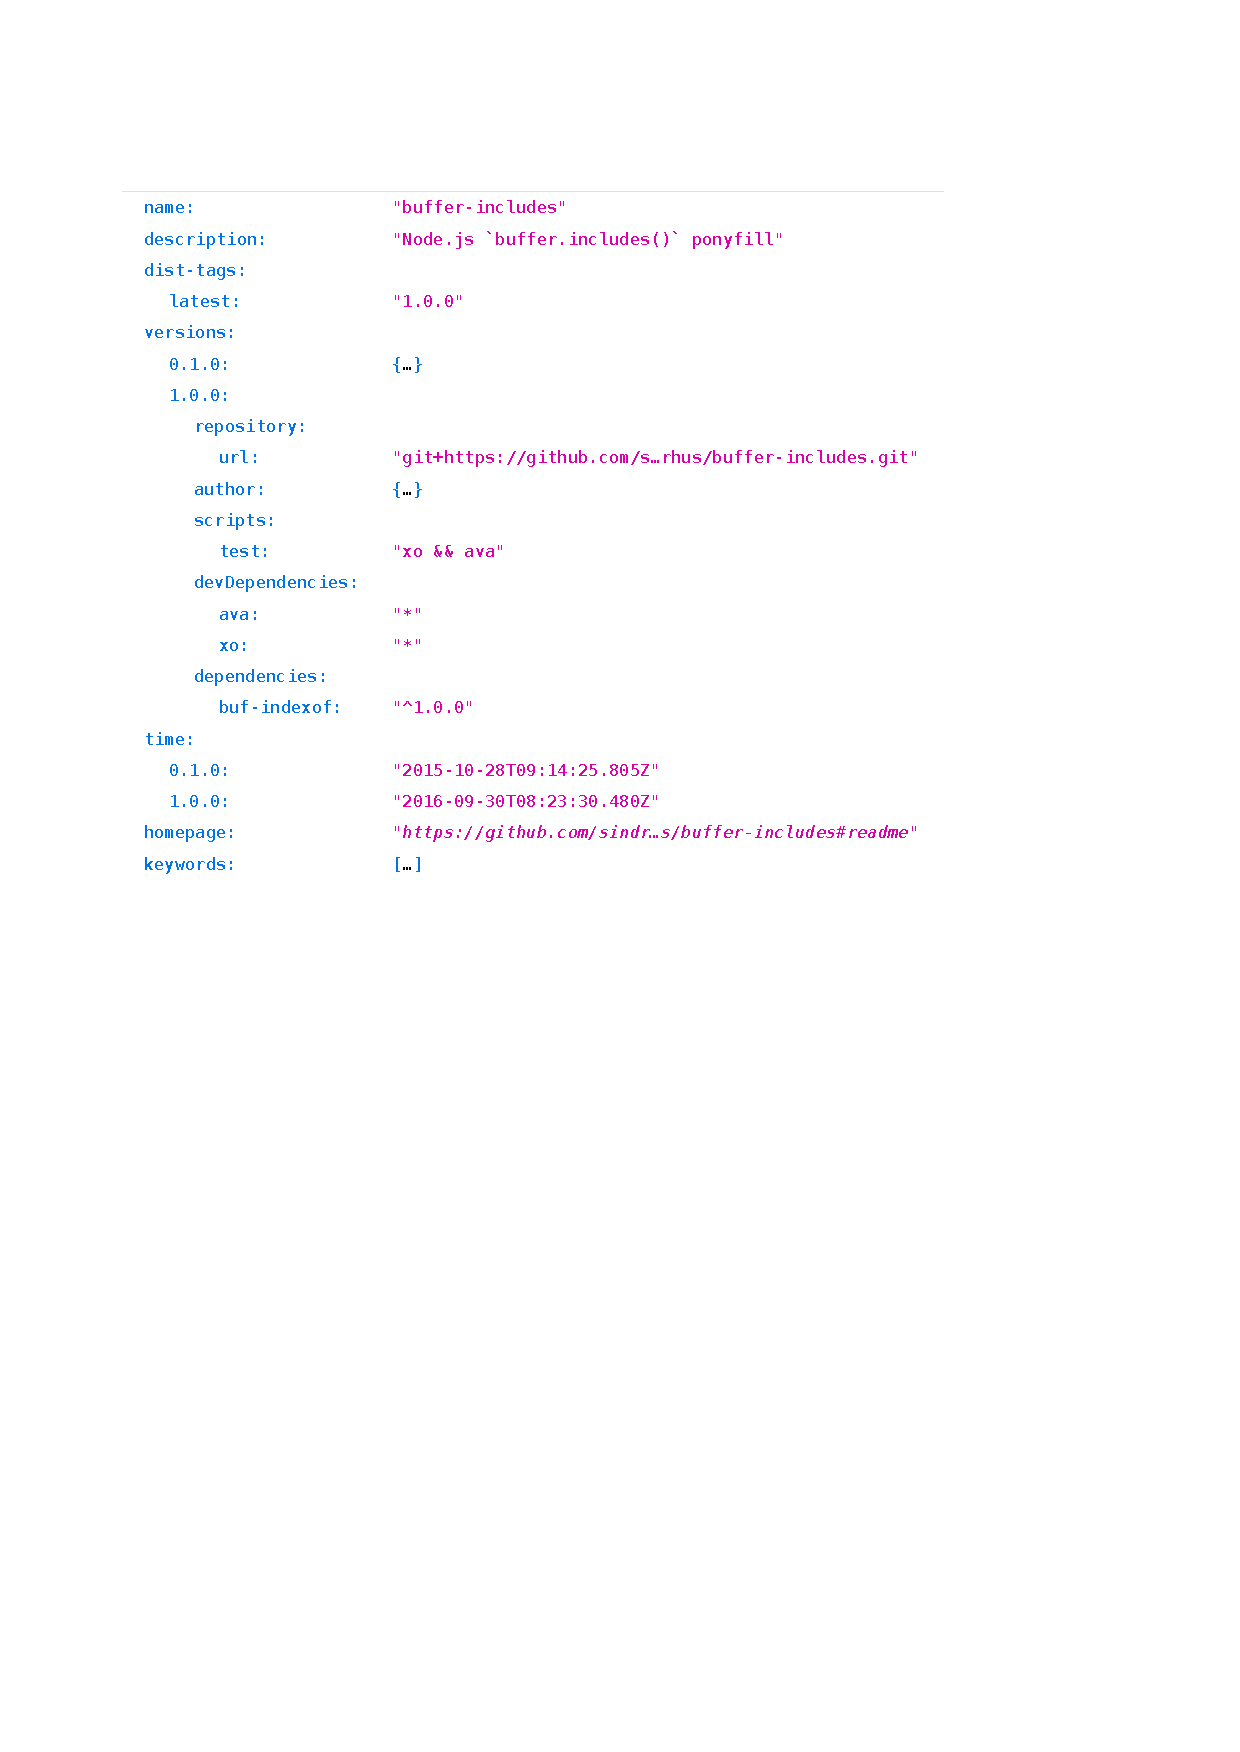
\includegraphics[scale=0.65]{figuras/package_json.pdf}
    \caption{Informações que serão recuperadas do \textit{package.json} para validar um pacote.}
    \label{fig:package_json}
\end{figure}{}

Foram excluídos desse conjunto de dados todos os pacotes que não continham nenhum provedor, pois quando um pacote não contém provedores não há como ser impactado por \textit{breaking changes}. Dessa maneira, o conjunto de dados final foi reduzido para um total de 987,595 pacotes clientes do \textsf{npm}. Por fim, para cada \textit{release} de todos os clientes, foram resolvidas as versões de todos os provedores com base no \textit{timestamp} dessa \textit{release}. Ou seja, foi resolvido o \textit{range} do provedor, que o cliente especificou naquela \textit{release}, para a maior versão aceita no momento da \textit{release} do cliente. Desse modo, foi determinada qual a versão do provedor o cliente utilizava no momento da publicação da \textit{release}.

\section{Amostra do Conjunto de Dados}
\label{sec:col_amostra}
% para remover a lista de siglas, foi utilizado um \textit no http
Para gerar a amostra utilizada neste trabalho, foram verificados dois requisitos nos \textit{987k} pacotes: 1) possuir um \textit{script} de teste não vazio e diferente do \textit{script} padrão de teste do \textsf{npm}: \texttt{\{"test": "Error: no test specified"\}} (488,805 conferem); e possuir a \textit{url} do repositório (410,433 conferem). Esses dois requisitos foram analisados na última \textit{release} disponível do pacote. Então, foi recuperada uma amostra representativa com 95\% de confiança e 5\% de margem de erro. Dentre os 410,433 pacotes restantes, a amostra resultou em 384 pacotes para serem analisados neste trabalho.

Foi realizada uma verificação manual nos repositórios do pacotes com menos de 4 \textit{releases} (130 dentre 384) para verificar se cada pacote não era um \textit{toy package}, ou seja, um pacote que não foi criado para ser um projeto real, apenas um teste no \textsf{npm}, no \textsf{GitHub} ou algo do tipo. Um pacote foi classificado como \textit{toy package} e foi removido, e outro foi sorteado seguindo os dois requisitos citados acima.

\section{Metodologia para Detecção de \textit{Breaking Changes}}
\label{sec:bcdetect}
Para este trabalho, foi desenvolvida uma ferramenta chamada \textsf{BCDetect}\footnote{https://github.com/danielventurini/bcdetect} disponível no \textsf{GitHub} sob a licença \textsf{MIT}. Esta ferramenta clona o repositório do respectivo cliente -- todos os clientes estavam hospedados no \textsf{Github} -- e cria uma estrutura de dados para armazenar as informações sobre o cliente. Nessa estrutura, cada \textit{release} do cliente contém todos os provedores com suas versões resolvidas e o tipo de atualização que os provedores realizaram desde a última \textit{release} do cliente: \texttt{steady} significa que o provedor não publicou nenhuma \textit{release} aceita desde a última release do cliente; \texttt{upgrade} significa que o provedor publicou uma nova \textit{release} aceita desde a última \textit{release} do cliente; e quando não há nenhuma dessas informações, o provedor foi inserido no \textit{package.json} nesta \textit{release}. Essa estrutura básica está representada na Figura \ref{fig:bc_work}, que seria construída a partir dos dados do cliente \textsf{buffer-includes} da Figura \ref{fig:package_json}.

\begin{figure}
    \centering
    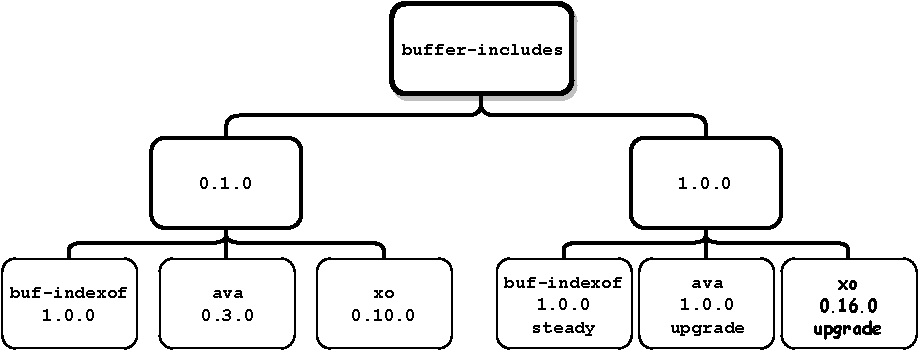
\includegraphics[scale=0.9]{figuras/bcdetect_work.pdf}
    \caption{Estrutura de dados para representar o cliente \textsf{buffer-includes}.}
    \label{fig:bc_work}
\end{figure}{}

Os testes de cada \textit{release} do cliente foram executados toda vez que havia pelo menos um provedor com nova \textit{release} (\textit{upgrade}) ou um provedor havia sido adicionado naquela \textit{release} do cliente. Após clonado o repositório, foi executado o comando \texttt{git checkout} para todas as \textit{releases} do cliente -- \textit{release} por \textit{release} -- com a respectiva \textit{tag} da \textit{release}, fazendo com que todos os arquivos sejam restaurados para exatamente os mesmos arquivos do momento em que o cliente publicou a \textit{release}. Uma \textit{tag} é uma referência a um ponto importante e específico do repositório, que geralmente são as \textit{releases}. Para \textit{releases} que o desenvolvedor não criou uma \textit{tag}, o \textit{checkout} foi realizado usando o \textit{timestamp} da respectiva \textit{release}. Em seguida, o arquivo \textit{package-lock.json}\footnote{https://docs.npmjs.com/files/package-lock.json} foi excluído, pois esse arquivo altera o comportamento do comando \texttt{npm install} -- a partir do \textsf{npm@5} -- fazendo com que o \textsf{npm} instale as versões dos provedores de acordo com o \textit{package-lock.json}, e não de acordo com o \textit{package.json}. Em sequência, todos provedores no \textit{package.json} e suas respectivas versões foram adicionados apenas no campo \textit{dependencies} do \textit{package.json} e os demais campos foram removidos,\footnote{campos para dependências no \textit{package.json}, tais como o \textit{peerDependencies}, \textit{optionalDependencies} e o \textit{globalDependencies}} uma vez que para executar os testes, ambos os provedores são requeridos.

O \textsf{Node.js} é o ambiente de execução para os pacotes \textsf{JavaScript} e a cada 6 meses uma nova \textit{release major} é publicada.\footnote{https://github.com/nodejs/node\#release-types} Por isso, antes de executar os testes da \textit{release} do cliente, a versão do \textsf{Node.js} precisa ser alterada. O chaveamento das \textit{releases} do \textsf{Node.js} é necessário pois as \textit{releases major} do \textsf{Node.js} não são retrocompatíveis, ou seja, um pacote que executa com sucesso na versão \textit{0.x} do \textsf{Node.js}, por exemplo, provavelmente não executaria com sucesso na versão \textit{8.x}. Para cada \textit{release} do cliente que teria seus testes executados, a versão do \textsf{Node.js} foi selecionada de duas maneiras: 1) do campo \texttt{engines->node} no \textit{package.json}, que permite o desenvolvedor especificar a versão do \textsf{Node.js}; e 2) através do \textit{timestamp} da \textit{release} do cliente, foi possível identificar a última \textit{release} do \textsf{Node.js} disponível,\footnote{https://nodejs.org/en/download/releases} ou seja, qual era a \textit{release} máxima do \textsf{Node.js} que os testes dos cliente foram executados no momento da \textit{release} do cliente. Assim, os testes do cliente foram executados em todas as versões \textit{major} do \textsf{Node.js}, da versão mais atual, pelo \textit{timestamp} da \textit{release} do cliente, até a versão \textit{major} mais antiga, ou até o teste ocorrer com sucesso. Para o cliente da Figura \ref{fig:bc_work}, a sua \textit{release 0.1.0} possui o \textit{timestamp} como \textit{2015-10-28}, e a última \textit{release} do \textsf{Node.js} disponível até esta data é a \textit{4.2.1}. Assim, os testes dessa \textit{release} do cliente seriam executados com as \textit{releases 4.x, 3.x, 2.x, 1.x, 0.x} do \textsf{Node.js}. Ao atualizar a \textit{release} do \textsf{Node.js}, a versão do \textsf{npm} é atualizada também. Isso é necessário pois é o \textsf{npm} que executa os \textit{scripts install} e \textit{test}. Após executar o \textit{install} e o \textit{test}, foram salvas as seguintes informações:

\begin{itemize}
    \item versão do cliente;
    \item se houve alteração na versão aceita de alguns dos provedores;
    \item os códigos da execução do \texttt{npm install} e \texttt{npm test} -- sucesso ou erro;
    \item a versão do \textsf{Node.js} que deveria ser executado com base na data da \textit{release}; e
    \item a versão do \textsf{Node.js} que os testes do cliente executaram com sucesso.
\end{itemize}{}

Os passos resumidos das operações em cada cliente juntamente com a verificação de alteração dos provedores e execução dos testes das \textit{releases} se encontram na Figura \ref{fig:steps_work}.

\begin{figure}
    \centering
    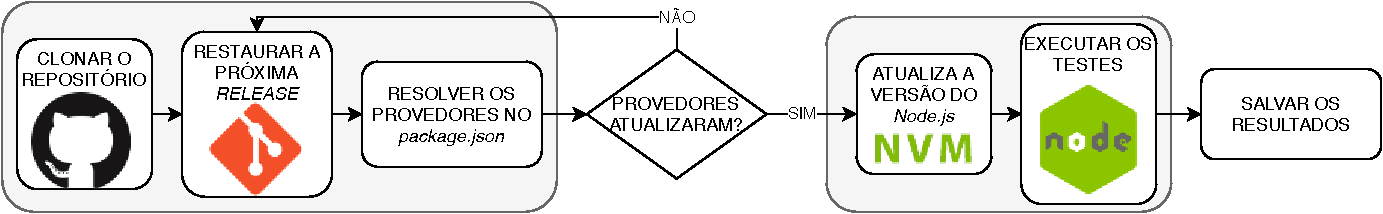
\includegraphics[scale=0.7]{figuras/steps_work.pdf}
    \caption{Etapas para clonar, restaurar e execução os testes das \textit{releases} de um cliente}
    \label{fig:steps_work}
\end{figure}{}

Dos 384 clientes que tiveram seus testes executados, em 33 não foi possível executar o comando \texttt{npm install}/\texttt{test} para nenhuma de suas \textit{releases}. Desses 33 clientes, 15 não possuíam algum dos arquivos necessários para os testes; 11 continham \textit{scripts} de teste inválidos em todas as suas \textit{releases}, tal como \texttt{\{"test": "no tests"\}}; 4 haviam listados alguns dos arquivos no \textit{.gitignore} -- arquivo utilizado pelo \textsf{git} para ignorar arquivos no repositório --, mas que eram necessários para a execução dos testes; 2 necessitaram de configurações específicas em banco de dados e não foi possível realizá-las; e 1 cliente requeria uma variável de ambiente para acessar um determinado site. Dessa forma, os 33 clientes foram substituídos em um novo sorteio seguindo o mesmo critério do sorteio anterior citado na Seção \ref{sec:col_amostra}, totalizando 384 clientes com 5957 \textit{releases} que foram utilizados no estudo.% Um detalhe importante refere-se aos clientes que utilizavam algum tipo de sistemas de banco de dados como o \textsf{MySql}. Quando um erro foi ocasionado pela falta de uma configuração básica, tal como executar um \textit{script} para criar uma tabela, então essas configurações foram realizadas e os testes do cliente foram re-executados. Somente quando o cliente necessitava de uma configuração específica e que não foi possível realizá-la, o cliente foi substituído por outro.

\subsection{Resultados da Execução dos Testes dos Clientes}
\label{sec:col_dados}

Após os comandos \texttt{npm install/test} executarem em pelo menos uma \textit{release} de todos os 384 clientes, 203 resultaram em erros para alguma de suas \textit{releases}. Analisando os resultados por \textit{releases}, de todas as 5957 \textit{releases}, foram executadas os testes de um total de 3230 \textit{releases}, enquanto que 2727 \textit{releases} não tiveram seus testes executados pois não haviam alterações nas \textit{releases} dos provedores, ou não continham algum \textit{script} de teste válido. Após o término da execução, 1954 \textit{releases} resultaram em sucesso, enquanto que 1276 \textit{releases} resultaram em erros no \textit{script install/test}. A Tabela \ref{tab:res_rq1_1} contém os resultados prévios sem que os clientes que resultaram em erro fossem analisados, ou seja, são dados apenas da execução dos testes dos clientes.

\begin{table}[]
\centering
\begin{tabular}{lrr}
\toprule
                    & Clientes & \textit{Releases} \\ \hline
    Total           & 384     & 5957     \\
    Não executado   & 0       & 2727     \\
    Executado       & 384     & 3230     \\
    Sucesso         & 181     & 1954     \\
    Erro            & 203     & 1276     \\ \bottomrule
\end{tabular}

\caption{Resultado da execução dos testes nas \textit{releases} de cada cliente, por clientes e por \textit{releases}.}
\label{tab:res_rq1_1}
\end{table}

% Após executarem, todas as 1276 \textit{releases} que resultaram em erros foram analisadas manualmente para separar os erros falso-positivos dos erros reais. Conforme explicado na Seção \ref{sec:qp1:approach}, os erros do tipo falso-positivos são erros que foram gerados pela falta de alguma configuração, isso é, devido uma má configuração, a execução dos testes da \textit{release} resultou em erros. Os erros falso-positivos mais comuns estavam relacionados a serviços que necessitavam de configurações prévias, tais como o \textsf{mysql} e o \textsf{mongodb}, que por vezes necessitavam de tabelas, senhas, \textit{scripts}, entre outras configurações para que os clientes executassem com sucesso seus testes. Após as \textit{releases} serem analisadas manualmente, foi constatado um total de 38 clientes com falso-positivos em todas as suas \textit{releases}, totalizando 172 \textit{releases} e mais 244 \textit{releases} que impactaram parcialmente outros clientes, ou seja, não foram o único tipo de erro no clientes. Assim, todos os 38 clientes e as 416 \textit{releases} foram consideradas como se os testes estivessem executados com sucesso. Dessa maneira, após a análise prévia, os dados atualizados são mostrados na Tabela \ref{tab:res_rq1_2} e na Figura \ref{fig:res_rq1_g}.

%\begin{table}[]
%\centering
%\begin{tabular}{lrr}
%\toprule
%                    & Clientes & \textit{Releases} \\ \hline
%    Sucesso         & 191     & 1388     \\
%    Erro            & 193     & 912     \\ \bottomrule
%\end{tabular}
%\caption{Resultado da execução dos testes, contabilizando os falso-positivos, por clientes e \textit{releases}.}
%\label{tab:res_rq1_2}
%\end{table}

%\begin{figure}
%    \centering
%    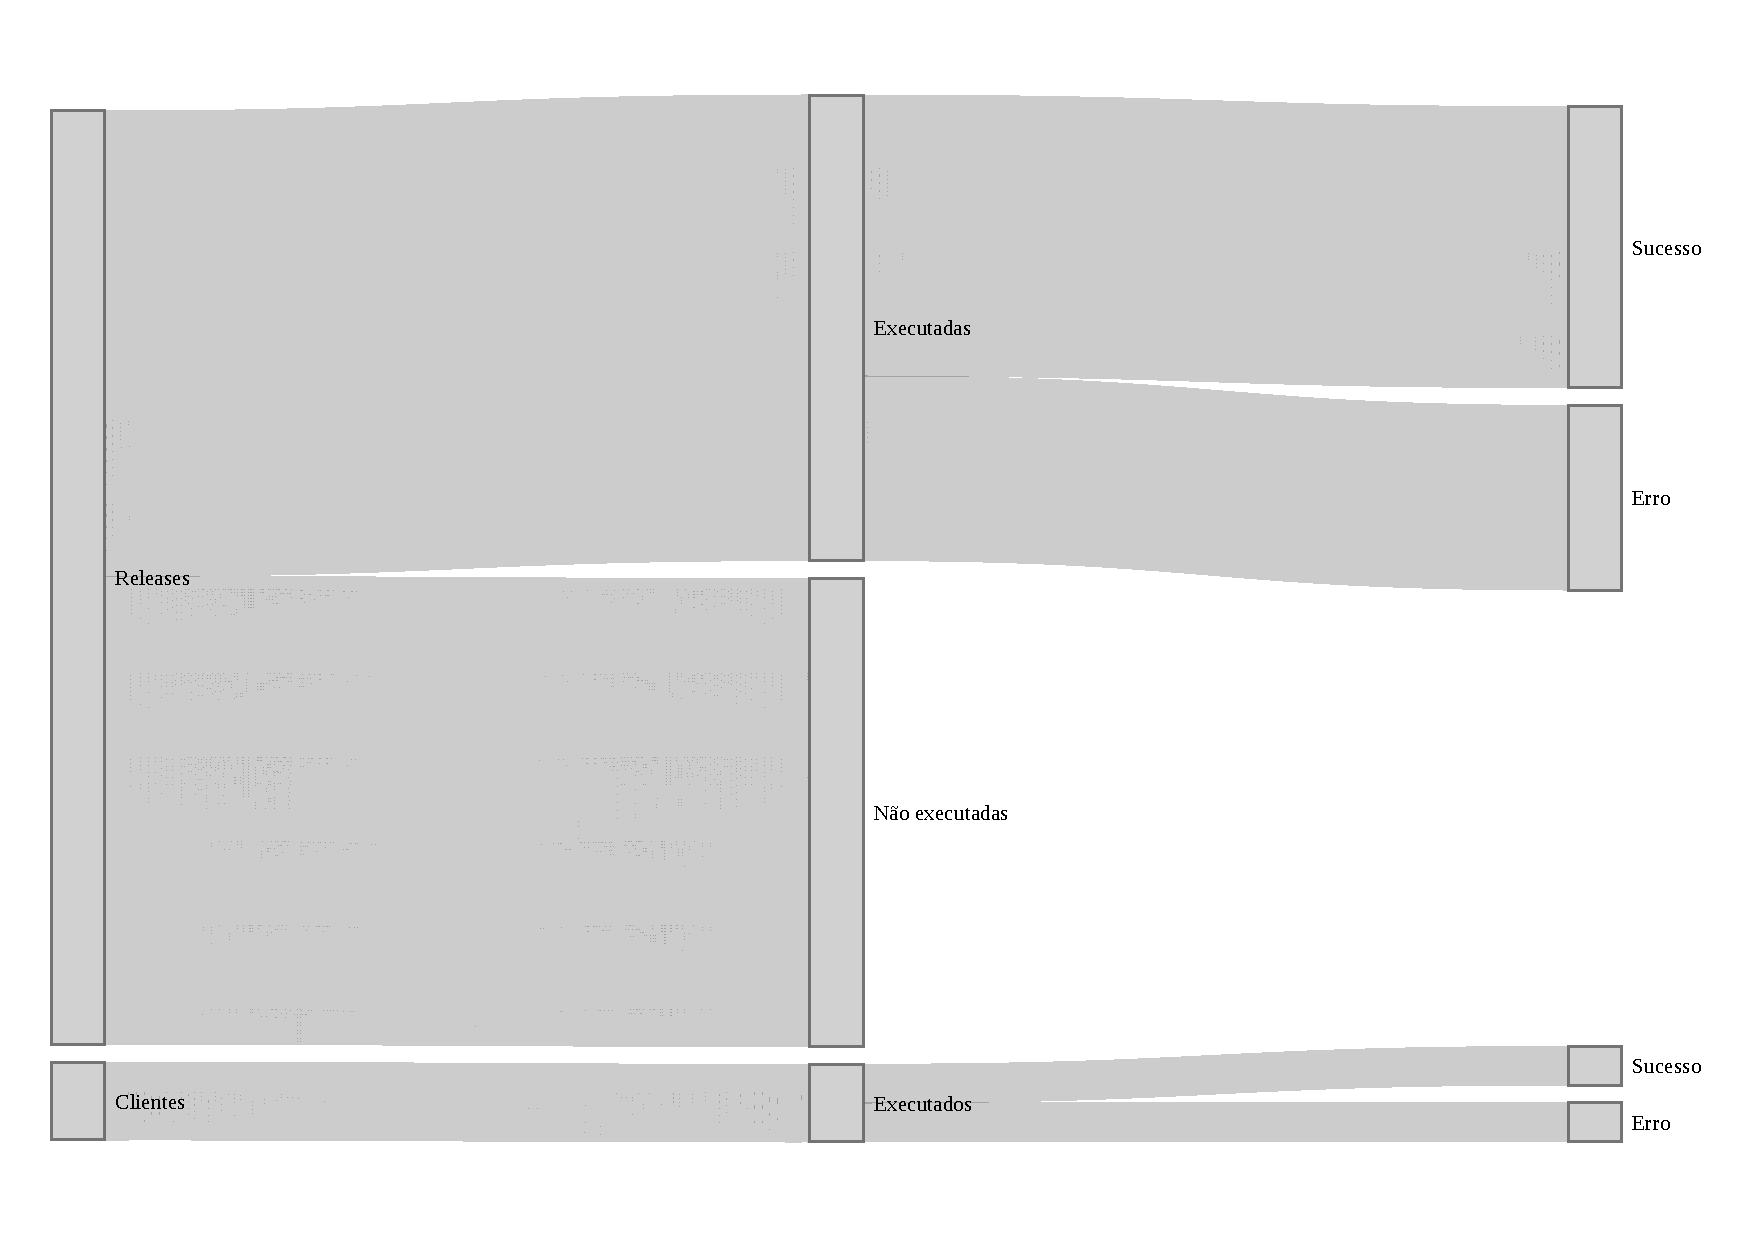
\includegraphics[scale=0.5]{figuras/general_results.pdf}
%    \caption{Resultado da execução dos testes, por clientes e por \textit{releases}.}
%    \label{fig:res_rq1_g}
%\end{figure}{}

Um pacote de replicação incluindo a amostra utilizada neste trabalho, as ferramentas, \textit{scripts} e todos os casos de \textit{breaking changes} está disponível no \textit{Zenodo}.\footnote{COMING: https://doi.org/10.44444/zenodo.99999999}